%!TEX root = ../report.tex
\section{Risk assessment}
The system is confronted by several risks which are determined and mitigated in this section.
The risk management involves : the identifcation of the risks, their probability and potential impact or consequences.

%Risk impact assesment and Prioritization
% Probability of Occurrence ( In the appendice is the table to which show how to evaluate a risk and the severity of consequences 
%http://www.mitre.org/publications/systems-engineering-guide/acquisition-systems-engineering/risk-management/risk-impact-assessment-and-prioritization % COSTS
Timeframe is classified in : Long , Medium , Short , Imminent \\
Consequences are classified in : Low, Moderate , High , Severe

\todo{Static path to local image}
%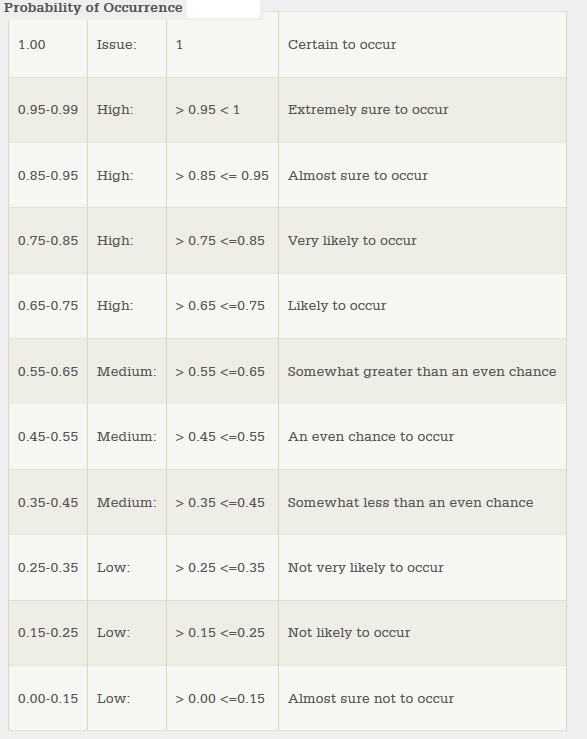
\includegraphics[scale=0.5]{C:/Users/admin/Desktop/M1/RISKSOCCURENCE.jpg} % maybe in the appendice ?
\subsection{Techincal}

	\textbf{ T-RISK1 The warning system does not detect floods in time.} \\
	\textit{Probability of Occurence} : Low \\ %because the system is supposed to be realiable 
	%Timeframe
	\textit{Consequences}: Severe because of the loss of human lives and money (estimate how much ?),loss of credibility regarding the end-users.\\
	\textit{Prevention}: Make sure the number of sensors is sufficient and that they are in good state (as low failure rate as possible : repaire or replace them ) thanks to a weekly checking for example. \\
	And that the system is available and reliable : it has to be checked and tested often.\\
	\textit{Decision} \\
	

	\textbf{ T-RISK2 The system sends warnings of a non-excising flood (false positive.} \\
	\textit{Probability of Occurence} : Low \\
	%Timeframe
	\textit{Consequences}: Moderate . People become more negligent to future messages. \\
	\textit{Prevention}: UAV's watching the area where the supposed flood is.\\
	Hiring an operator to control . \\
	\textit{Decision}: Send a message as soon as the mistake is detected to tell the population it was a false alert. \\
	

	\textbf{ T-RISK3 The system can't send messages to the necessary people because the communication platform is also destroyed by the flood.} \\
	\textit{Probability of Occurence} :MEDIUM\\
	%Timeframe
	\textit{Consequences} : Severe . No warning sent or too late => Loss of human lives and money .\\
	\textit{Prevention}: Find another way to get the phone number of a population (?). \\
	\textit{Decision} : Using other medias : television, radio, Intenet , ... \\
	

	\textbf{ T-RISK4 The system sends incorrect information, causing extra damage.} \\
	\textit{Probability of Occurence} :LOW\\
	%Timeframe
	\textit{Consequences} : High . Loss of money and maybe lives.\\
	\textit{Prevention}: Operator checking the validity of the information sent by the system.\\
	Good collaboration with the insurance companies. \\
	%\textit{Decision}: \\

	\textbf{ T-RISK5 Hacker get access to the system} \\
	\textit{Probability of Occurence}:LOW \\
	\textit{Consequences} : High. The hackers may sent incorrect information deliberately during the flood : Loss of money and maybe human lives. The system isn't realiable anymore. \\
	\textit{Prevention}: Change password and hashcodes every six months. \\
	\textit{Decision} : Update the security system / change it. Find a new algorithm for the creation of password and hascodes. \\


\subsection{Business}

	\textbf{ B-RISK1 Wrong estimation of the budget} \\
	\textit{Probability of Occurence} :Medium \\
	%Timeframe
	\textit{Consequences} : High . The final product hasn't the features expected. \\
	\textit{Prevention} : The team needs an accountant or at least someone taking care of the follow-up of the money. \\
	\textit{Decision} : Remove some requirements or features of the product. \\

	\textbf{ B-RISK2 The money invested in the fabrication and achievement of the product/system isn't "covered" by the sales (shortfall/deficit)} \\
	\textit{Probability of Occurence}:Medium \\
	%Timeframe
	\textit{Consequences}: High .Stopping the sale \\
	%\textit{Prevention}: 
	\textit{Decision} : Adding more features to the product in order to make it more competitive in the market. \\
	

	\textbf{ B-RISK3 Competitors lowering their prices so our company has to reduce its} \\
	\textit{Probability of Occurence}: Medium \\
	%Timeframe
	\textit{Consequences} : Moderate . Loss of money \\
	%\textit{Prevention} \\
	%\textit{Decision} \\
	
	\textbf{ B-RISK4 The sensors company become bankrupt} \\
	\textit{Probability of Occurence}: Low \\
	\textit{Consequences}: High.\\
	\textit{Prevention} Our system use sensors from different companies \\
	\textit{Decision}: Find another company selling sensors and make sure of its reliability. \\


\subsection{Schedule}

	\textbf{ S-RISK1 The project isn't finished at the deadline} \\
	\textit {Probability of Occurence}  : Low
	%Timeframe
	\textit{Consequences} : Pressure for all the team members, loss of credibility regarding the end-users, selling a product with less fetures than expected.\\
	\textit{Prevention} : Meeting for the team members every week to keep track of the timing and take decisions according to the deadline. \\
	\textit{Decision} : Remove some requirements or features in order to finish the project as soon as possible.\\